\documentclass{beamer}
\usetheme{Berlin}  %% Themenwahl
\usecolortheme{beaver}

\usepackage{listings}
\usepackage{graphicx}
\usepackage{hyperref}
\usepackage[utf8]{inputenc}
\usepackage{amssymb}
\usepackage{amsmath}
\usepackage{esvect}
%\usepackage{mcode}
 
\title{Ray Tracing Optimization - Plan vs. Reality}
\author{Kashofer, Radschek}
\date{\today}

\begin{document}
\maketitle
\frame{\tableofcontents[currentsection]}
 
\section{Plan}
\begin{frame}
	\begin{quote}If you want to make god laugh, tell him your plans.\end{quote}
\end{frame}
\begin{frame} %%Eine Folie
	\frametitle{The way to hell is paved with good intentions} %%Folientitel
	\begin{columns}
	\begin{column}{0.5\textwidth}
  	\begin{figure}
		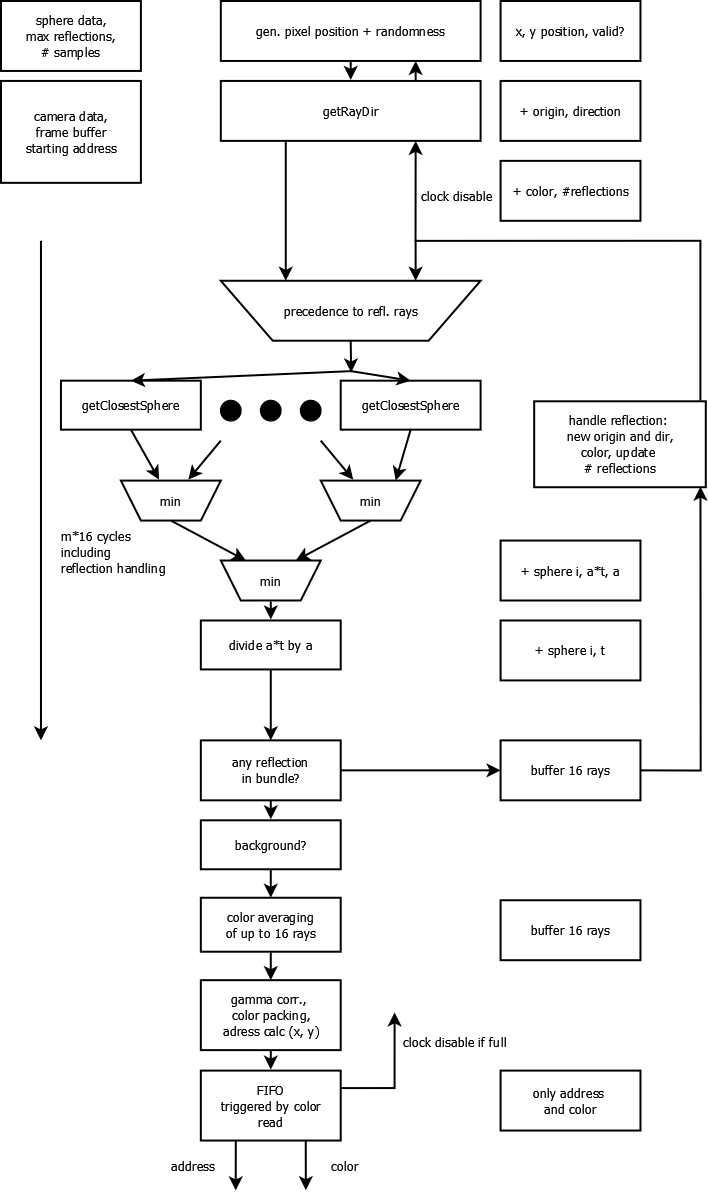
\includegraphics[height=0.8\textheight]{pics/pipe.png}
		\caption{PipelineDesign}
	\end{figure}
	\end{column}
	\begin{column}{0.5\textwidth}
		\begin{itemize}
			\item<2->split up work for 3 group members
			\item<3->implement individual parts
			\item<4->fit together for great pipeline
			\item<5->write software
			\item<6-> ???
			\item<7->PROFIT!
			\begin{figure}
				
\includegraphics[height=0.3\textheight]{pics/Gnomes_plan.png}
			\end{figure}
		\end{itemize}
	\end{column}
	\end{columns}
\end{frame}

\section{Obstacles}
\begin{frame} %%Eine Folie
	\frametitle{} %%Folientitel
  	\begin{itemize}
			\item time to say good bye \pause  - to Florian
			\pause
			\item compiling \pause - where did my quartus go?
			\pause
			\item basic arithmetic \pause- 3 cycles plus one addition equals ... a number
			\pause
			\item general philosophical questions \pause - "what makes a cycle 'even'"?
			\pause
			\item the sheer number of side information you have to keep track of
		\end{itemize}
\end{frame}

\section{Status}
\begin{frame} %%Eine Folie
	\frametitle{New Design} %%Folientitel
	\begin{figure}
		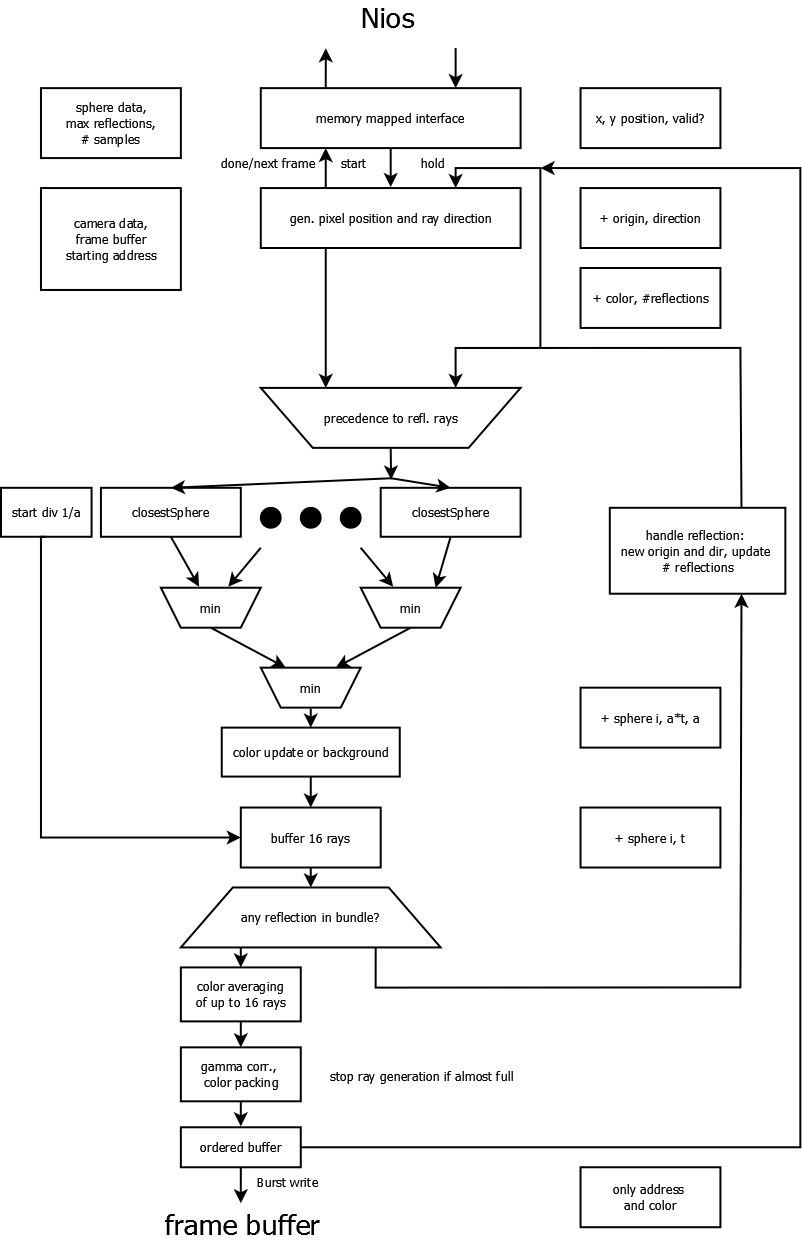
\includegraphics[height=0.8\textheight]{pics/pipeNeu.png}
	\end{figure}
  \end{frame}

\begin{frame} %%Eine Folie
	\frametitle{New Design} %%Folientitel
	Ok, it looks almost the same, BUT:
	\begin{itemize}
		\item merged functions that need same data\\ \pause
			original approach too close to SW, not feasible
		\pause
		\item removed need for stall\\ \pause
		stalling a pipeline (without messing everything up) is hard!\\ \pause
		new approach allows all rays in pipeline to be finished
		\pause
		\item buffer at the end is now ordered by address\\ \pause  
		(reduces buffer size by a factor of 2)
		\pause
		\item we talk directly to the frame buffer \\ \pause
		removes bottleneck nios
	\end{itemize}
	
\end{frame}

  	\begin{frame} %%Eine Folie
	\frametitle{Nothing works} %%Folientitel
	\begin{itemize}
		\item all the parts exists
		\pause
		\item they do not fit together (yet - but we're getting there)
		\pause
		\item overhead for carrying data along is MUCH higher than expected \\
		\pause
		(especially for the coding monkey...)
	\end{itemize}
\end{frame}

\section{Lessons Learnt}

\begin{frame} %%Eine Folie
	\frametitle{} %%Folientitel
	\begin{itemize}
		\item Counting to 2 is harder than it looks
		\pause
		\item You WILL forget vital information and redo port interfaces constantly
		\pause
		\item Do not upset your quartus gods
		\pause
		\item teamwork is hard.
	\end{itemize}
\end{frame}


\end{document}